\section{ChIRP. Robot}
\label{sec:chirp}
The ChIRP (CHeap and Interchangable Robotic platform) robot is a robot developed by the CRAB lab, which is part of the artificial intelligence group at the Department of Computer and Information Science (IDI) at the Norwegian University of Science And Technology (NTNU).

The purpose behind the development of the ChIRP robot is to research sub symbolic AI, i.e. both  swarming or evolution. Sub symbolic AI are algorithms and AI inspired by nature or biology. E.g Artificial Neural Network inspired from the human brain and swarm robots inspired from bird flocks, ant colonies, fish schools and bees. Evolution and genetic programming are also one of topics included in sub symbolic AI.
The robot's data schema and source code are all open source and can be found at \href{http://chirp.idi.ntnu.no}{chirp.idi.ntnu.no}. The robot consist of a \textbf{printed circuit board (PCB)}, two motors which controls the two wheels on each side of the robot.
Modules like LED lights and various sensors can be soldered on the PCB thus the robots' are easily modifiable, and the robots can have multiple layers with different sensors so it is not limited to have only light sensors or infrared sensors. The standard ChIRP robot comes with eight infrared-LEDs and eight infrared receivers as seen on figure \ref{fig:chirpAbove}. As seen in figure \ref{fig:chirpmod}, the robot have two extra layers added with light sensors. Other layers with other types of sensors can easily be added at will on these ChIRP robots.
\begin{figure}[H]
\centering
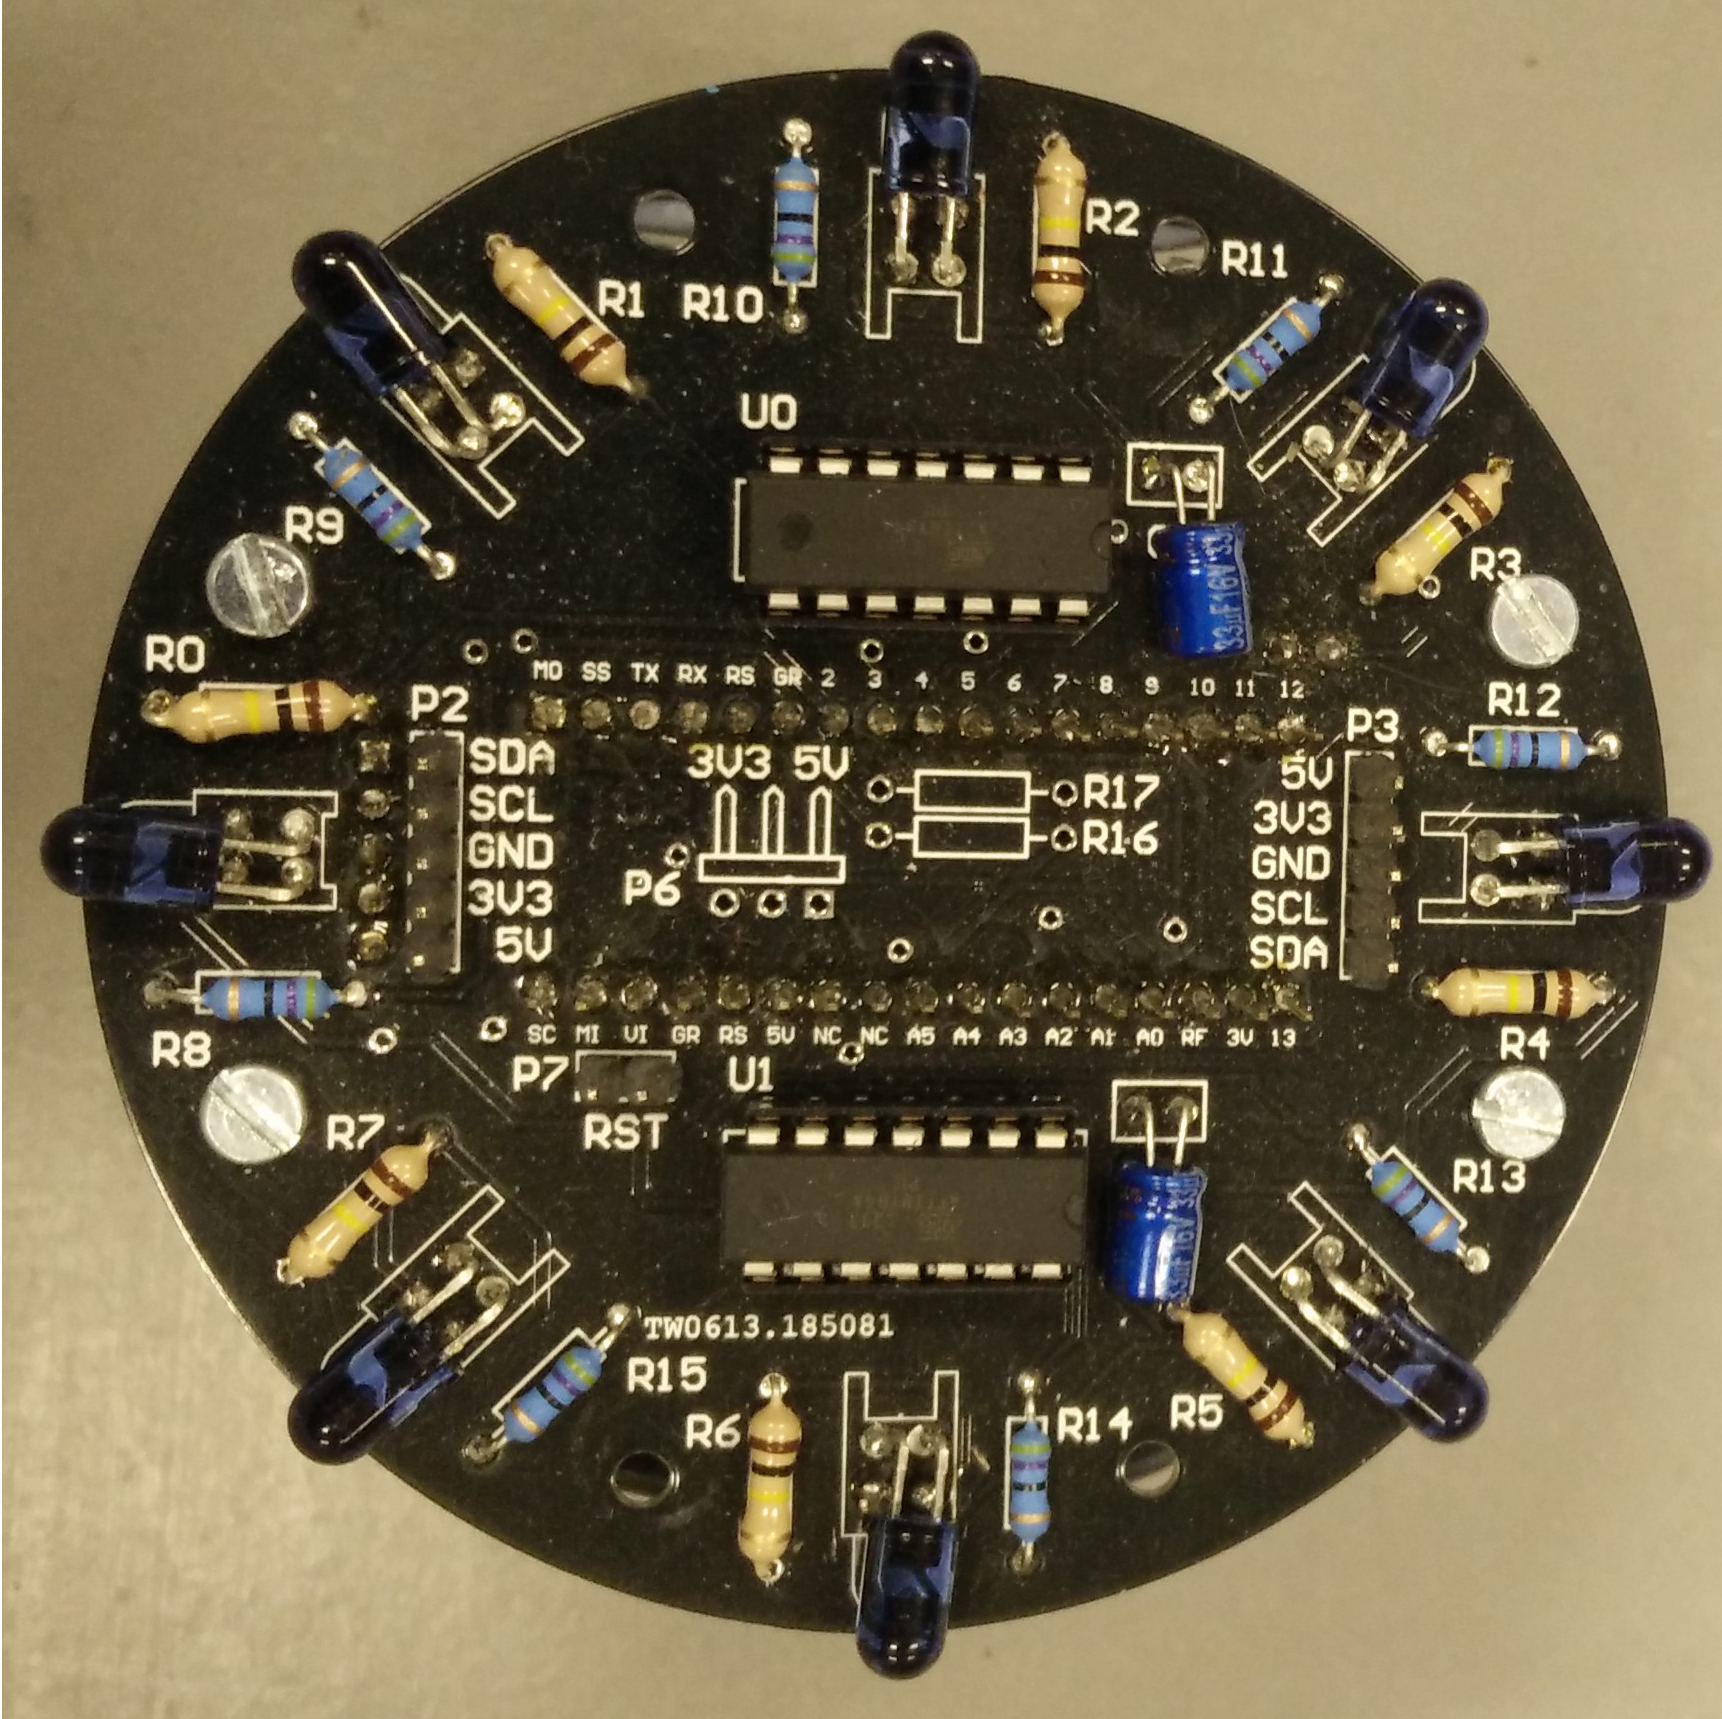
\includegraphics[width=0.8\linewidth]{images/chirpAbove.jpg}
\caption[ChIRP robot seen from above]{ChIRP robot seen from above, this one is equipped with eight infrared emitters and receivers}
\label{fig:chirpAbove}
\end{figure}
These can be used to measure distance by emitting the infrared light and measure how much of it is reflected back into the receiver. There are two ATtiny on top of the robot. ATtiny are a very simple microcontroller made by Atmel. These ATtiny are programmed to handle the values found by measuring the resistance from the infrared filtered resistor, and convert them to a short (16 bit int) so the Arduino micro inside the ChIRP does not need to handle everything by itself. This is due to the limited processor power of the Arduino micro which has a ATmega32u4 processor with 16 MHz clock speed and 32 KB flash memory. Arduino micro has 20 digital inpput/output (I/O) pins in which 7 of them are PWM, and 12 analog input pins. PWM stands for Pulse-width modulation \footnote{\href{http://arduino.cc/en/Tutorial/PWM}{http://arduino.cc/en/Tutorial/PWM}}, and those pins with PWM are able to emulate analog output by variating the high and low signal with various speed, also called modulation.
\begin{figure}[H]
\centering
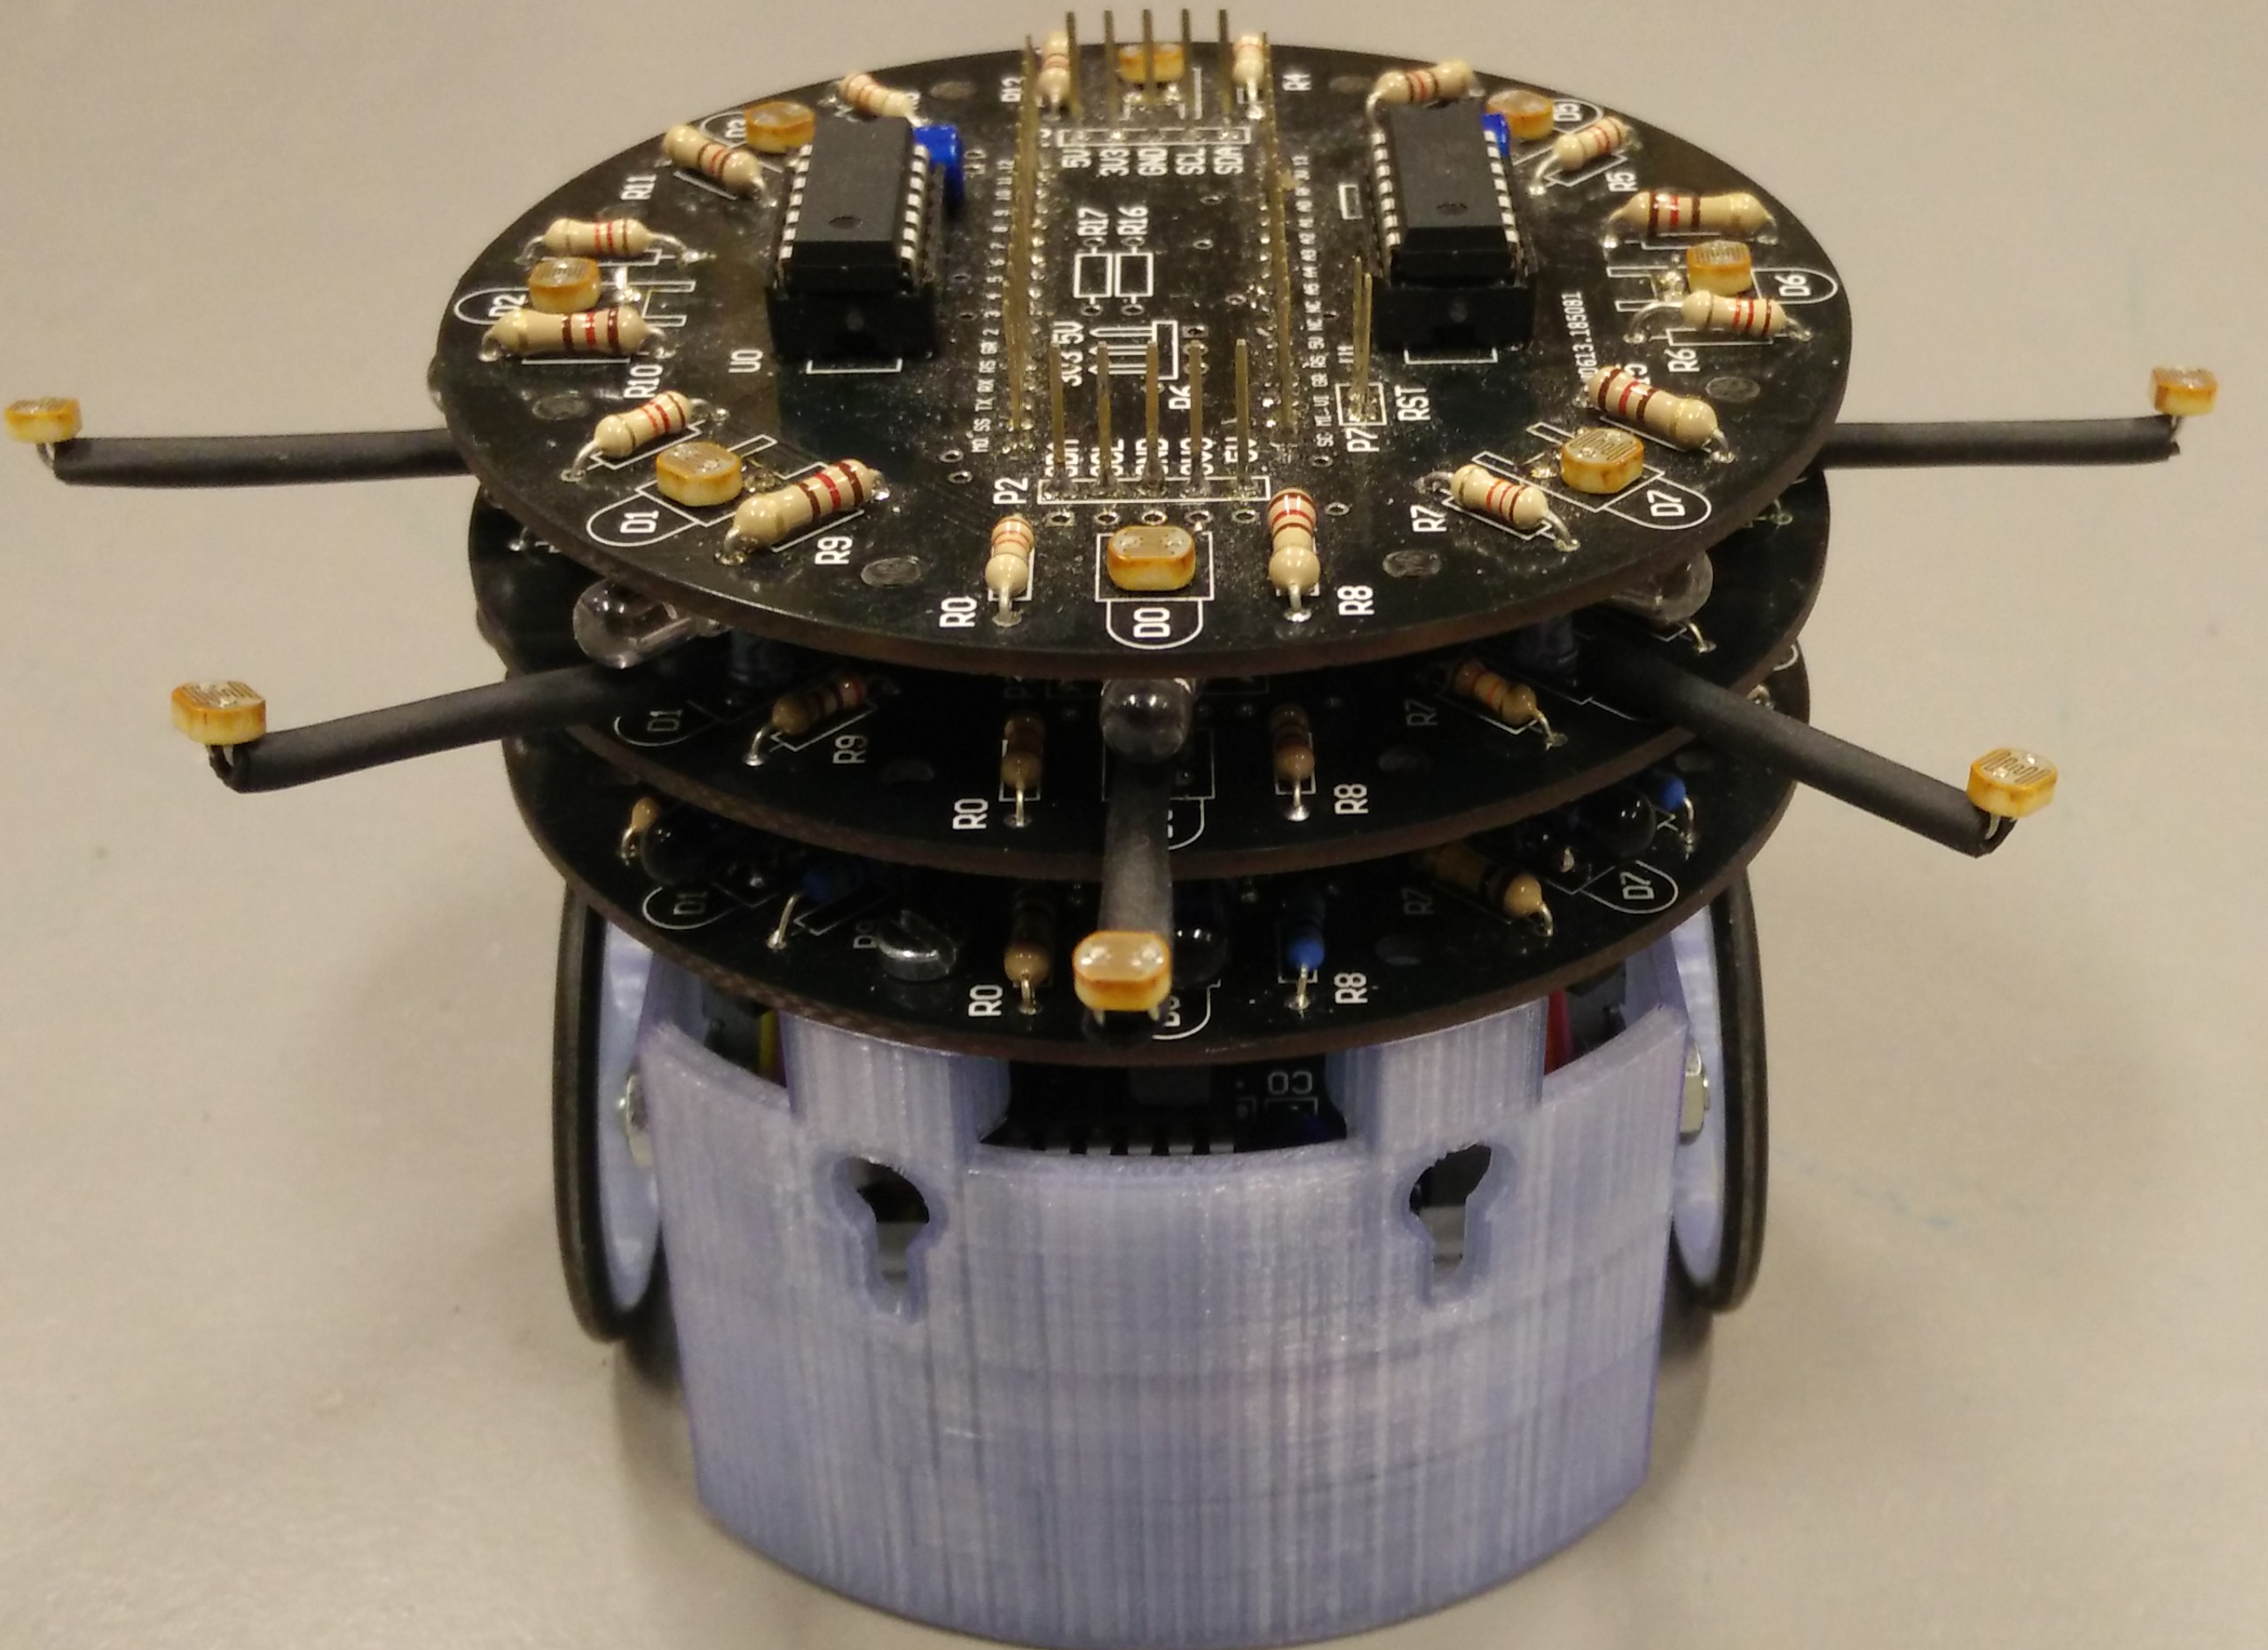
\includegraphics[width=0.8\linewidth]{images/chirpModified}
\caption[Modified ChIRP]{A modified ChIRP robot with extra light sensors}
\label{fig:chirpmod}
\end{figure}

Inside the robot there's an ATtiny as well that helps the Arduino control the motors. These ATtinys that controls the motors and the 8 infrared receiver sensors needs to be programmed. The code is also available on the website. These ATtinys can be programmed using an Arduino Uno shield or by connecting the Uno to the ATtiny using a breadboard directly.
\begin{figure}[H]
	\centering
	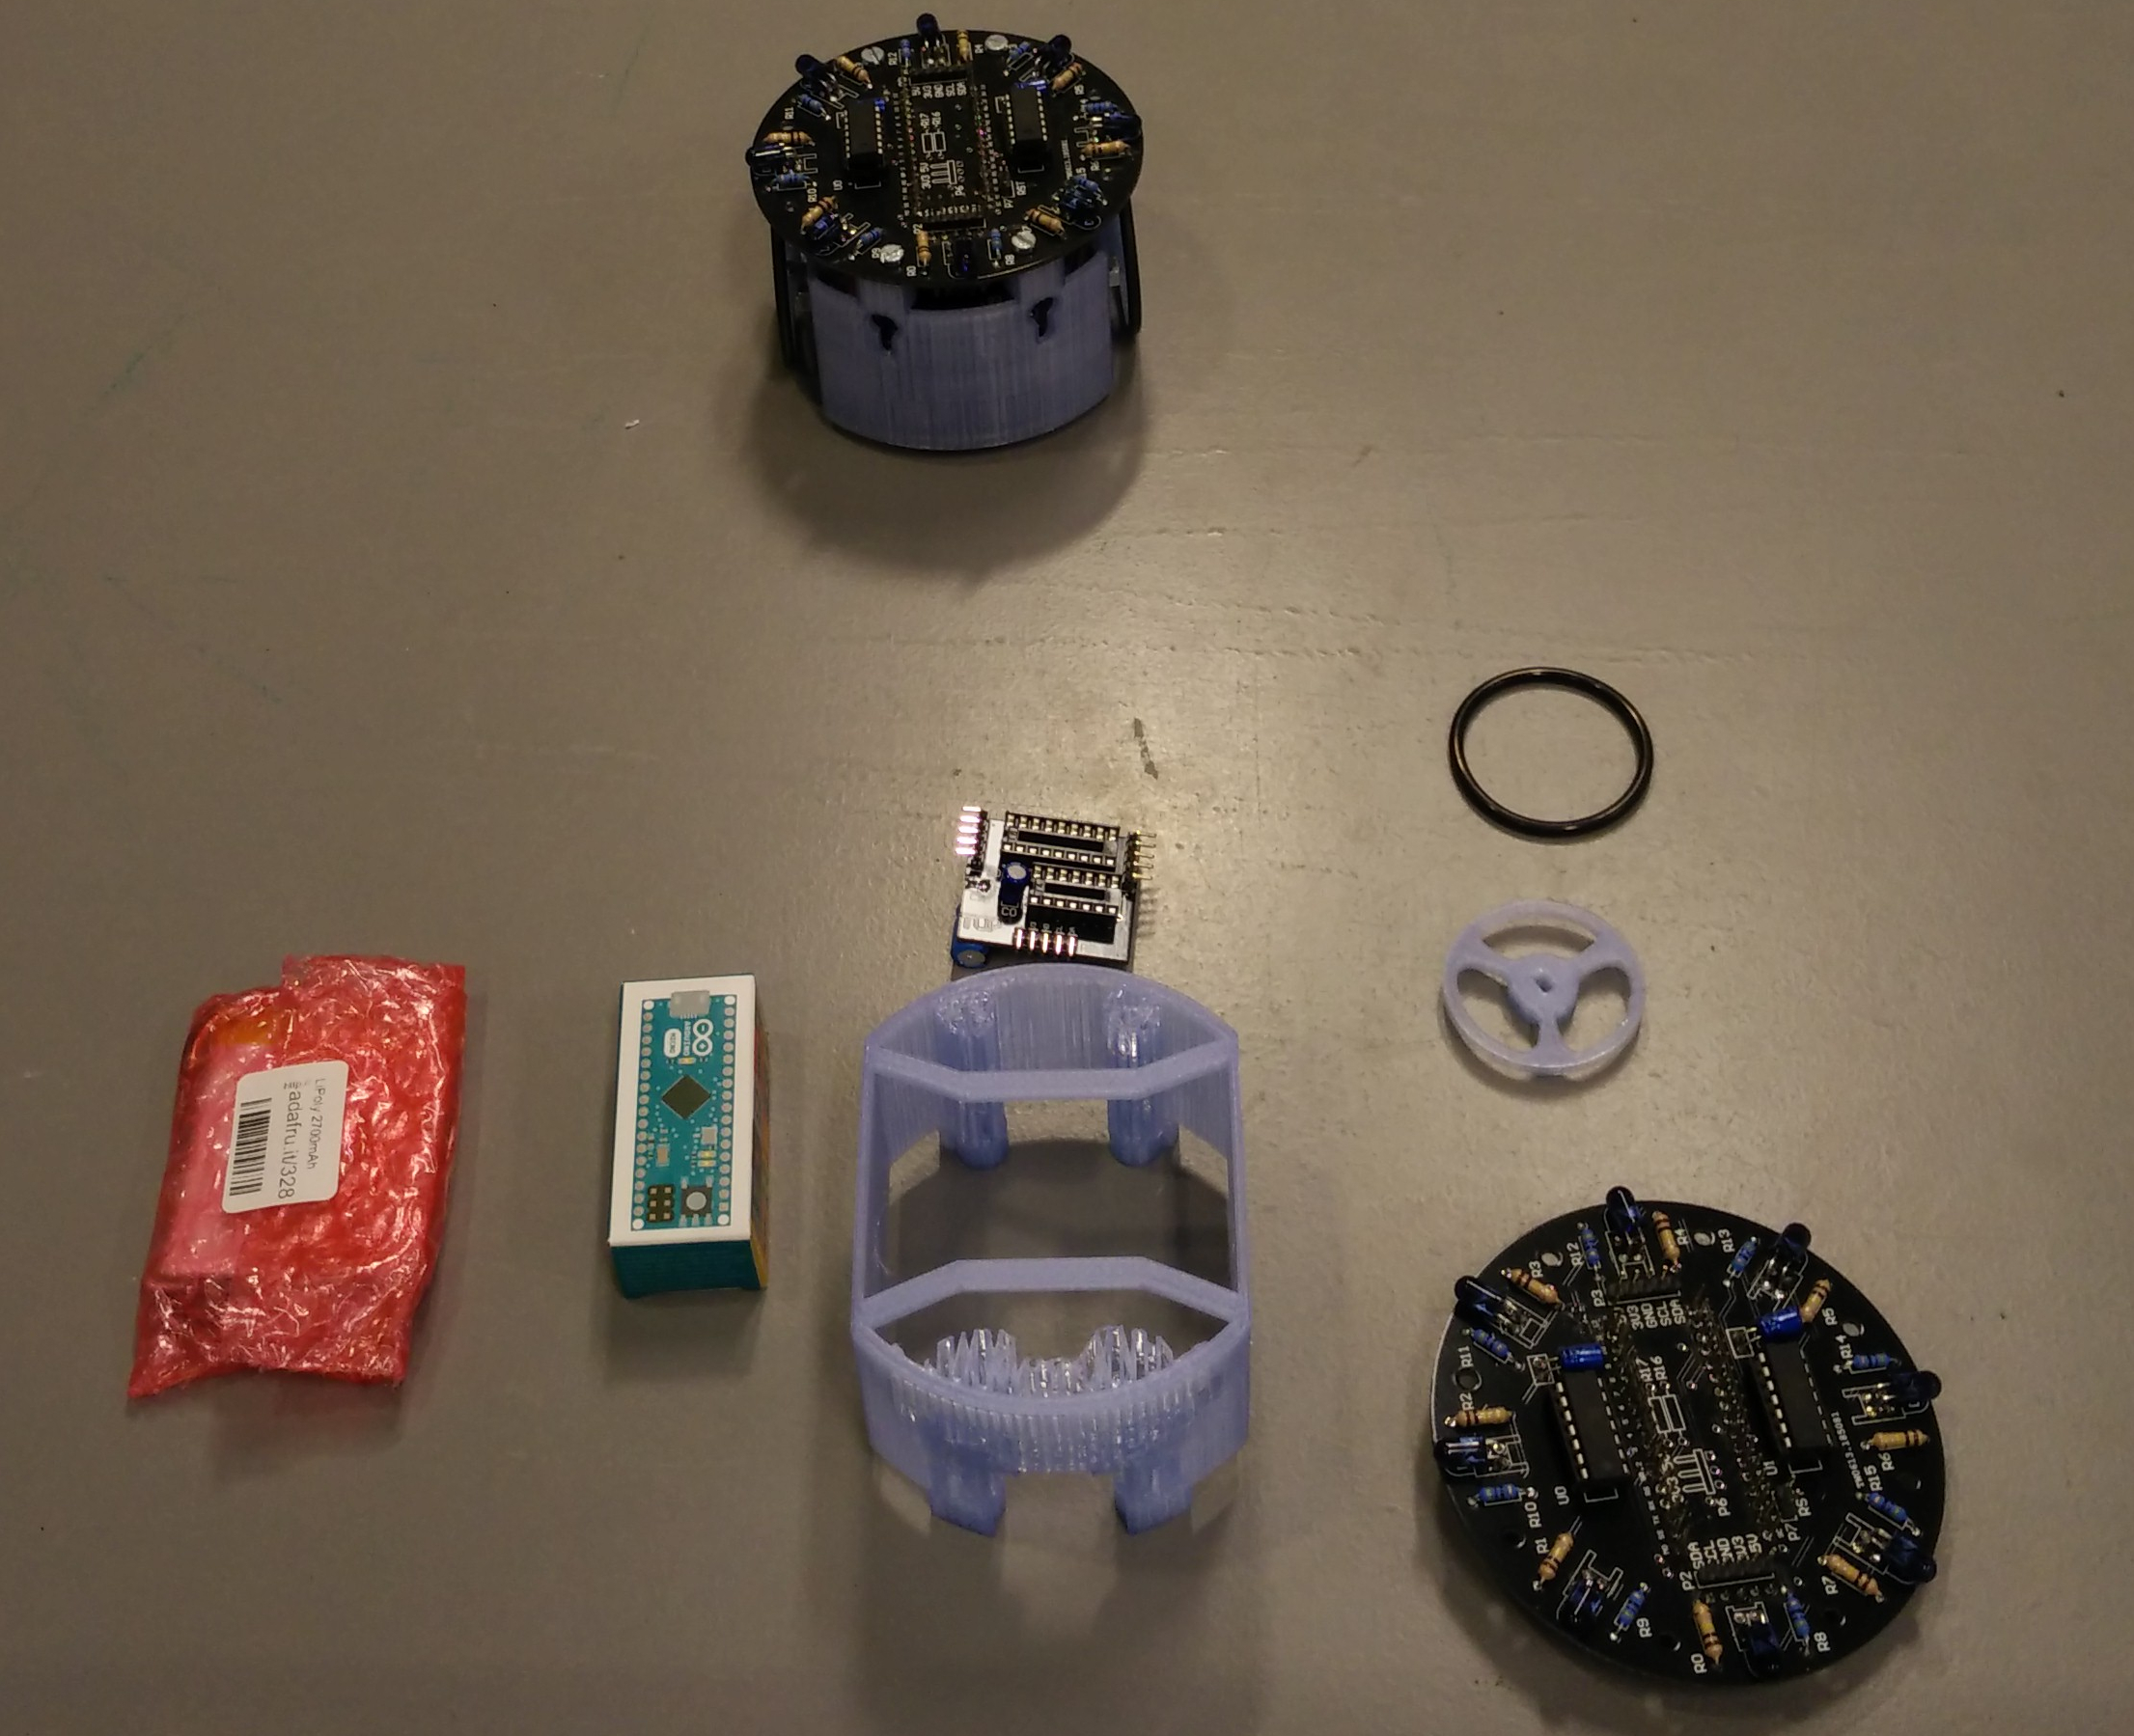
\includegraphics[width=0.8\linewidth]{images/chirpPieces}
	\caption[ChIRP pieces]{Some of the building blocks of the chirp robot}
\end{figure}

The ChIRPs are powered by a 3.7 volts 2500mAh battery which lasts for about 4.5 hours if they are running continuously, and it takes around 4 hours to recharge. The battery life can be increased if the robot is standing still. The batteries can be changed, but it can be quite difficult to do so due to the small gaps and the precision needed to connect the wires. The robots can be charged using a normal micro USB cable.




